\documentclass[aps,prx,twocolumn,superscriptaddress,nofootinbib]{revtex4-2}
\usepackage{amsmath,amssymb,bm}
\usepackage{graphicx}
\usepackage{hyperref}

% Auto-generated by generate_bt2t001_paper_assets.py -- DO NOT EDIT BY HAND
\newcommand{\btProtocolId}{\texttt{OSIRIS-BT2T-001-FEZ}}
\newcommand{\btExperimentBaseId}{\texttt{OSIRIS-BT2T-001}}
\newcommand{\btCardId}{\texttt{Card A}}
\newcommand{\btBackend}{\texttt{ibm\_fez}}
\newcommand{\btJobId}{\texttt{dc2ee3uq4uuc73a56o6g}}
\newcommand{\btExecTier}{\texttt{HARDWARE\_ATTESTED}}
\newcommand{\btEncVer}{\texttt{bt2t-enc-1}}
\newcommand{\btEncSha}{\texttt{3e3b02d13539daaf}}
\newcommand{\btQpySha}{\texttt{81a90cf823da78f2}}
\newcommand{\btRawGzSha}{\texttt{b3be6057b50a9223}}
\newcommand{\btPreregSha}{\texttt{513f55909f613c0d}}
\newcommand{\btGoneSha}{\texttt{f543aa9613469e34}}
\newcommand{\btCalSnapSha}{\texttt{f6316b95b1023389}}
\newcommand{\btBtPySha}{\texttt{e179cfb1cd431615}}
\newcommand{\btCapsuleSha}{\texttt{c6ce4301304ddeab}}
\newcommand{\btQpuSec}{11}
\newcommand{\btResUnits}{0.1678}
\newcommand{\btQuotaLimitSec}{600}
\newcommand{\btQuotaRemBeforeSec}{19}
\newcommand{\btQuotaRemAfterSec}{8}
\newcommand{\btNumQubits}{5}
\newcommand{\btHilbertDim}{32}
\newcommand{\btGroupOrder}{24}
\newcommand{\btUnusedCount}{8}
\newcommand{\btFixedTotal}{10}
\newcommand{\btTranspositions}{11}
\newcommand{\btAssocTriples}{13,824}
\newcommand{\btLayoutStr}{[21, 22, 23, 16, 24]}
\newcommand{\btReadoutOrderStr}{[24, 16, 22, 23, 21]}
\newcommand{\btHubQubit}{23}
\newcommand{\btCalScore}{0.01502}
\newcommand{\btCalCzSum}{0.00921}
\newcommand{\btCalRoMean}{0.00852}
\newcommand{\btCalSxMean}{0.00031}
\newcommand{\btCalScoreRoWeight}{0.5}
\newcommand{\btCalScoreSxWeight}{5.0}
\newcommand{\btCalMinToneUs}{80}
\newcommand{\btCalMinTtwoUs}{50}
\newcommand{\btNumBlocks}{3}
\newcommand{\btPubsPerBlock}{96}
\newcommand{\btTotalPubs}{288}
\newcommand{\btMaxPubsLimit}{300}
\newcommand{\btShotsPerPub}{96}
\newcommand{\btShotsPerCell}{288}
\newcommand{\btTotalShots}{27,648}
\newcommand{\btShotsPerArm}{9,216}
\newcommand{\btShotsValidPerArm}{6,912}
\newcommand{\btShotsUnusedPerArm}{2,304}
\newcommand{\btCalWindows}{1}
\newcommand{\btShotRetentionPct}{100\%}
\newcommand{\btTranspilerSeed}{20261122}
\newcommand{\btScheduleSeed}{20261123}
\newcommand{\btLogGenX}{48}
\newcommand{\btLogGenCx}{32}
\newcommand{\btLogGenMcx}{11}
\newcommand{\btLogGenDepth}{56}
\newcommand{\btLogGenErr}{3.47 \times 10^{-14}}
\newcommand{\btLogStructX}{8}
\newcommand{\btLogStructCx}{6}
\newcommand{\btLogStructCcx}{1}
\newcommand{\btLogStructMcx}{1}
\newcommand{\btLogStructDepth}{8}
\newcommand{\btLogStructErr}{3.55 \times 10^{-15}}
\newcommand{\btSuperposErr}{1.90 \times 10^{-14}}
\newcommand{\btStageZeroErr}{1.31 \times 10^{-14}}
\newcommand{\btAtaStructCz}{48}
\newcommand{\btAtaStructDepth}{168}
\newcommand{\btAtaStructSize}{242}
\newcommand{\btAtaGenCz}{400}
\newcommand{\btAtaGenDepth}{1,481}
\newcommand{\btAtaGenSize}{2,069}
\newcommand{\btAtaCzRatio}{8.33\times}
\newcommand{\btTfOptOneStructCz}{84}
\newcommand{\btTfOptOneStructDepth}{268}
\newcommand{\btTfOptOneGenCz}{838}
\newcommand{\btTfOptOneGenDepth}{2,736}
\newcommand{\btStructCz}{72}
\newcommand{\btStructSx}{151}
\newcommand{\btStructRz}{117}
\newcommand{\btStructX}{10}
\newcommand{\btStructDepth}{218}
\newcommand{\btStructSize}{350}
\newcommand{\btStructInitIdx}{[2, 0, 3, 1, 4]}
\newcommand{\btStructFinalIdx}{[4, 3, 1, 2, 0]}
\newcommand{\btGenCz}{723}
\newcommand{\btGenSx}{1,560}
\newcommand{\btGenRz}{956}
\newcommand{\btGenX}{42}
\newcommand{\btGenDepth}{2,073}
\newcommand{\btGenSize}{3,281}
\newcommand{\btGenInitIdx}{[4, 1, 0, 3, 2]}
\newcommand{\btGenFinalIdx}{[1, 2, 0, 4, 3]}
\newcommand{\btCtrlCz}{0}
\newcommand{\btCtrlSx}{0}
\newcommand{\btCtrlDepth}{0}
\newcommand{\btCzRatioTf}{10.04\times}
\newcommand{\btSxRatioTf}{10.33\times}
\newcommand{\btDepthRatioTf}{9.51\times}
\newcommand{\btTkStructZzOpt}{47}
\newcommand{\btTkStructDepthOpt}{194}
\newcommand{\btTkStructSizeOpt}{294}
\newcommand{\btTkStructZzRaw}{48}
\newcommand{\btTkGenZzOpt}{400}
\newcommand{\btTkGenDepthOpt}{1,720}
\newcommand{\btTkGenSizeOpt}{2,520}
\newcommand{\btTkGenZzRaw}{428}
\newcommand{\btTkZzRatio}{8.51\times}
\newcommand{\btHOneThresh}{0.25}
\newcommand{\btHOneBlockAlpha}{0.01}
\newcommand{\btHTwoDeltaThresh}{0.20}
\newcommand{\btHTwoLeakThresh}{0.15}
\newcommand{\btHThreeSpamThresh}{0.90}
\newcommand{\btRandChance}{0.03125}
\newcommand{\btRandChanceFour}{0.0312}
\newcommand{\btRandLeakBase}{0.25}
\newcommand{\btPValidStructRaw}{0.5337}
\newcommand{\btPValidStructSe}{0.0059}
\newcommand{\btPValidStructSd}{0.0096}
\newcommand{\btPValidStructBlkZero}{0.5243}
\newcommand{\btPValidStructBlkOne}{0.5334}
\newcommand{\btPValidStructBlkTwo}{0.5434}
\newcommand{\btPValidStructMit}{0.6104}
\newcommand{\btPValidStructModal}{24}
\newcommand{\btLeakStruct}{0.0940}
\newcommand{\btStructSecCenter}{0.5035}
\newcommand{\btStructSecImag}{0.5214}
\newcommand{\btStructSecHurwitz}{0.5421}
\newcommand{\btPUnusedStructRaw}{0.5595}
\newcommand{\btPUnusedStructSe}{0.0100}
\newcommand{\btPUnusedStructSd}{0.0054}
\newcommand{\btPUnusedStructMit}{0.6070}
\newcommand{\btPUnusedStructModal}{8}
\newcommand{\btLeakUnusedToValidStruct}{0.1593}
\newcommand{\btStructModalAll}{32}
\newcommand{\btPValidGenRaw}{0.0661}
\newcommand{\btPValidGenSe}{0.0030}
\newcommand{\btPValidGenSd}{0.0065}
\newcommand{\btPValidGenBlkZero}{0.0694}
\newcommand{\btPValidGenBlkOne}{0.0586}
\newcommand{\btPValidGenBlkTwo}{0.0703}
\newcommand{\btPValidGenMit}{0.0715}
\newcommand{\btPValidGenModal}{11}
\newcommand{\btLeakGen}{0.2115}
\newcommand{\btGenSecCenter}{0.0764}
\newcommand{\btGenSecImag}{0.0666}
\newcommand{\btGenSecHurwitz}{0.0647}
\newcommand{\btPUnusedGenRaw}{0.0777}
\newcommand{\btPUnusedGenSe}{0.0056}
\newcommand{\btPUnusedGenSd}{0.0091}
\newcommand{\btPUnusedGenMit}{0.0792}
\newcommand{\btPUnusedGenModal}{5}
\newcommand{\btLeakUnusedToValidGen}{0.6797}
\newcommand{\btGenModalAll}{16}
\newcommand{\btPValidCtrlRaw}{0.8643}
\newcommand{\btPValidCtrlSe}{0.0040}
\newcommand{\btPValidCtrlSd}{0.0020}
\newcommand{\btPValidCtrlBlkZero}{0.8655}
\newcommand{\btPValidCtrlBlkOne}{0.8620}
\newcommand{\btPValidCtrlBlkTwo}{0.8655}
\newcommand{\btPValidCtrlMit}{1.0000}
\newcommand{\btPValidCtrlModal}{24}
\newcommand{\btLeakCtrl}{0.0330}
\newcommand{\btCtrlSecCenter}{0.8385}
\newcommand{\btCtrlSecImag}{0.8426}
\newcommand{\btCtrlSecHurwitz}{0.8757}
\newcommand{\btPUnusedCtrlRaw}{0.9076}
\newcommand{\btPUnusedCtrlSe}{0.0060}
\newcommand{\btPUnusedCtrlSd}{0.0034}
\newcommand{\btPUnusedCtrlMit}{1.0000}
\newcommand{\btPUnusedCtrlModal}{8}
\newcommand{\btCtrlModalAll}{32}
\newcommand{\btCtrlAllMean}{0.8751}
\newcommand{\btDeltaValidRaw}{0.4676}
\newcommand{\btDeltaValidMit}{0.5388}
\newcommand{\btBlkDeltaZero}{0.4549}
\newcommand{\btBlkDeltaOne}{0.4748}
\newcommand{\btBlkDeltaTwo}{0.4731}
\newcommand{\btPairedBlockT}{73.23}
\newcommand{\btPairedBlockP}{9.32 \times 10^{-5}}
\newcommand{\btElemWins}{24}
\newcommand{\btElemMinDelta}{0.3299}
\newcommand{\btElemMaxDelta}{0.6285}
\newcommand{\btWilcoxonP}{1.19 \times 10^{-7}}
\newcommand{\btDeltaUnusedRaw}{0.4818}
\newcommand{\btDeltaUnusedMit}{0.5279}
\newcommand{\btRoCond}{1.4524}
\newcommand{\btHOneVerdict}{\texttt{SUPPORTED}}
\newcommand{\btHTwoVerdict}{\texttt{SUPPORTED}}
\newcommand{\btHThreeVerdict}{\texttt{REFUTED}}
\newcommand{\btCalProdFid}{0.9580}
\newcommand{\btCalProdFidPct}{95.80\%}
\newcommand{\btMargPredValid}{0.8647}
\newcommand{\btMargPredUnused}{0.9063}
\newcommand{\btMargPredAll}{0.8751}
\newcommand{\btMargDiffValid}{4.3 \times 10^{-4}}
\newcommand{\btMargDiffAll}{7.0 \times 10^{-6}}
\newcommand{\btQTwentyFourCalPct}{0.33\%}
\newcommand{\btQTwentyFourLivePct}{4.92\%}
\newcommand{\btQTwentyFourErrZeroOnePct}{0.17\%}
\newcommand{\btQTwentyFourErrOneZeroPct}{9.66\%}
\newcommand{\btQTwentyFourStaleX}{14.91\times}
\newcommand{\btQSixteenCalPct}{0.79\%}
\newcommand{\btQSixteenLivePct}{1.06\%}
\newcommand{\btQSixteenStaleX}{1.34\times}
\newcommand{\btQTwentyTwoCalPct}{0.35\%}
\newcommand{\btQTwentyTwoLivePct}{0.28\%}
\newcommand{\btQTwentyTwoStaleX}{0.80\times}
\newcommand{\btQTwentyThreeCalPct}{0.44\%}
\newcommand{\btQTwentyThreeLivePct}{0.41\%}
\newcommand{\btQTwentyThreeStaleX}{0.94\times}
\newcommand{\btQTwentyOneCalPct}{2.34\%}
\newcommand{\btQTwentyOneLivePct}{6.33\%}
\newcommand{\btQTwentyOneErrZeroOnePct}{9.90\%}
\newcommand{\btQTwentyOneErrOneZeroPct}{2.76\%}
\newcommand{\btQTwentyOneStaleX}{2.70\times}

\newcommand{\btTableCompilationRows}{%
Logical Gate-Level & \texttt{GENERIC} (11 transpositions) & 32 \texttt{CX} + 11 \texttt{MCX} & --- & 91 & 56 & $\|U - P_{32}\|_\infty = 3.47 \times 10^{-14}$ \\
Logical Gate-Level & \texttt{STRUCTURED} (coset-parity) & 6 \texttt{CX} + 1 \texttt{CCX} + 1 \texttt{MCX} & --- & 16 & 8 & $\|U - P_{32}\|_\infty = 3.55 \times 10^{-15}$ \\
Qiskit All-to-All (opt 3) & \texttt{GENERIC} & 400 \texttt{CZ} & --- & 2,069 & 1,481 & Exact up to global phase \\
Qiskit All-to-All (opt 3) & \texttt{STRUCTURED} & 48 \texttt{CZ} & --- & 242 & 168 & Exact ($8.33\times$ \texttt{CZ} reduction) \\
Heavy-Hex \texttt{T5} (opt 1) & \texttt{GENERIC} / \texttt{STRUCTURED} & 838 / 84 \texttt{CZ} & --- & 3,992 / 400 & 2,736 / 268 & Exact ($9.98\times$ \texttt{CZ} reduction) \\
\texttt{ibm\_fez} \texttt{T5} Core (opt 3) & \texttt{GENERIC} & 723 \texttt{CZ} & 1,560 & 3,281 & 2,073 & 96/96 Stage-0 PASS ($\le 1.31 \times 10^{-14}$) \\
\texttt{ibm\_fez} \texttt{T5} Core (opt 3) & \texttt{STRUCTURED} & 72 \texttt{CZ} & 151 & 350 & 218 & Exact ($10.04\times$ \texttt{CZ} reduction) \\
Local \texttt{pytket} \texttt{H2} Rebase & \texttt{GENERIC} / \texttt{STRUCTURED} & 400 / 47 \texttt{ZZPhase} & --- & 2,520 / 294 & 1,720 / 194 & \texttt{PROXY} ($8.51\times$ \texttt{ZZPhase} reduction) \\
}

\newcommand{\btTableHardwareSummaryRows}{%
\texttt{STRUCTURED} (72 / 151 / 218) & $0.5337 \pm 0.0059$ & 0.0096 & 0.6104 & 0.5035 & 0.5214 & 0.5421 & $0.5595 \pm 0.0100$ & 0.0940 & 32/32 \\
\texttt{GENERIC} (723 / 1,560 / 2,073) & $0.0661 \pm 0.0030$ & 0.0065 & 0.0715 & 0.0764 & 0.0666 & 0.0647 & $0.0777 \pm 0.0056$ & 0.2115 & 16/32 \\
\texttt{PREP\_RO\_CTRL} (0 / 0 / 0) & $0.8643 \pm 0.0040$ & 0.0020 & 1.0000 & 0.8385 & 0.8426 & 0.8757 & $0.9076 \pm 0.0060$ & 0.0330 & 32/32 \\
}

\newcommand{\btTablePerQubitSpamRows}{%
$b_0$ & \texttt{q24} (LSB leaf) & 99.9 / 120.4 & 0.33\% & 4.92\% & 0.17\% & 9.66\% & $14.91\times$ \\
$b_1$ & \texttt{q16} (interior) & 148.5 / 122.3 & 0.79\% & 1.06\% & 0.54\% & 1.58\% & $1.34\times$ \\
$b_2$ & \texttt{q22} (interior) & 145.6 / 117.1 & 0.35\% & 0.28\% & 0.13\% & 0.43\% & $0.80\times$ \\
$b_3$ & \texttt{q23} (degree-3 hub) & 144.3 / 136.1 & 0.44\% & 0.41\% & 0.17\% & 0.65\% & $0.94\times$ \\
$b_4$ & \texttt{q21} (MSB leaf) & 201.6 / 159.5 & 2.34\% & 6.33\% & 9.90\% & 2.76\% & $2.70\times$ \\
}


\begin{document}

\title{Exact Binary Tetrahedral Group Inversion on a 5-Qubit Heavy-Hex Superconducting Register: Coset-Parity Synthesis Compression and Unflagged Readout Staleness}

\author{Devin Phillip Davis}
\affiliation{Agile Defense Systems LLC, Lexington, Kentucky, USA}
\date{November 23, 2026}

\begin{abstract}
Non-abelian finite-group primitives underpin discrete gauge-theory simulation and non-abelian quantum error-correcting codes, yet naive truth-table decompositions of finite-group operations compile into prohibitive multi-controlled entangling depths on sparse superconducting topologies. Under write-ahead preregistered protocol \btProtocolId\ (\btCardId, independent gate \texttt{G1} signed off prior to hardware submission), we implement exact group inversion $g \mapsto g^{-1}$ for the binary tetrahedral group $2T \subset SU(2)$ ($|2T| = \btGroupOrder$ Hurwitz quaternion units embedded in a $\btNumQubits$-qubit Hilbert space of dimension $\btHilbertDim$ with $\btUnusedCount$ fixed unused codewords under frozen encoding \btEncVer, SHA-256 prefix \btEncSha) on a five-transmon heavy-hex T-junction $\btLayoutStr$ of the 156-qubit IBM Heron~r2 processor \btBackend\ (job \btJobId, \btExecTier, \btTotalShots\ equal-shot physical measurements across \btTotalPubs\ ISA circuits in \btNumBlocks\ temporally interleaved blocks, \btQpuSec\,s QPU). Exploiting the normal quaternion subgroup decomposition $2T = Q_8 \rtimes \mathbb{Z}_3$, coset-parity Boolean factoring compresses heavy-hex \texttt{CZ} count by \btCzRatioTf\ from \btGenCz\ \texttt{CZ} (\btGenSx\ $\sqrt{X}$, unitary depth \btGenDepth) in the generic $\btTranspositions$-transposition reference to \btStructCz\ \texttt{CZ} (\btStructSx\ $\sqrt{X}$, unitary depth \btStructDepth) for the identical $32\times 32$ permutation unitary, and compresses local \texttt{pytket} \texttt{H2}-native compilation from \btTkGenZzOpt\ to \btTkStructZzOpt\ \texttt{ZZPhase} gates (\btTkZzRatio). Within this single attested calibration window ($N_{\mathrm{windows}} = \btCalWindows$), uniform valid-group raw inversion accuracy increases from $\widehat{P}_{\mathrm{valid\text{-}24}}(\mathrm{GENERIC}) = \btPValidGenRaw \pm \btPValidGenSe$ to $\widehat{P}_{\mathrm{valid\text{-}24}}(\mathrm{STRUCTURED}) = \btPValidStructRaw \pm \btPValidStructSe$ (\btPValidStructMit\ secondary readout-mitigated, $\mathrm{cond}(M_{32}) = \btRoCond$), yielding $\Delta\widehat{P}_{\mathrm{valid\text{-}24}} = +\btDeltaValidRaw$ (paired block $t_{\mathrm{df}=2} = \btPairedBlockT$, one-sided $p = \btPairedBlockP$; $\btElemWins / \btGroupOrder$ elementwise wins, exact two-sided Wilcoxon $p = \btWilcoxonP$; \texttt{H1} = \btHOneVerdict) and $\btStructModalAll / \btHilbertDim$ exact modal majority-vote recovery. Unused-codeword preservation improves by $+\btDeltaUnusedRaw$ ($\btPUnusedStructRaw$ versus $\btPUnusedGenRaw$) while confining valid-to-unused subspace leakage to $\btLeakStruct < \btHTwoLeakThresh$ below the $\btRandLeakBase$ uniform random baseline (\texttt{H2} = \btHTwoVerdict). Simultaneously, the interleaved \btCtrlCz-\texttt{CZ} preparation-and-readout control attains $\widehat{P}_{\mathrm{unused\text{-}8}} = \btPUnusedCtrlRaw \ge \btHThreeSpamThresh$ but $\widehat{P}_{\mathrm{valid\text{-}24}} = \btPValidCtrlRaw < \btHThreeSpamThresh$, honestly refuting \texttt{H3} (\btHThreeVerdict) and exposing an unflagged \btQTwentyFourStaleX\ live readout staleness excursion on leaf transmon \texttt{q24} (\btQTwentyFourCalPct\ published versus \btQTwentyFourLivePct\ live) alongside a \btQTwentyOneStaleX\ excursion on \texttt{q21} (\btQTwentyOneCalPct\ versus \btQTwentyOneLivePct).
\end{abstract}

\maketitle

\section{Introduction}
Discrete non-abelian subgroups of $SU(2)$ serve as tractable finite truncations of continuous $SU(2)$ Yang--Mills lattice gauge theories~\cite{LammLawrenceYamauchi2019,BenderZoharCirac2018} and provide group-algebraic substrates for non-abelian fault-tolerant primitives~\cite{MochxonKitaevPreskill2004,Barenco1995}. Among the polyhedral double covers in $SU(2)$, the binary tetrahedral group $2T \cong SL(2,\mathbb{F}_3)$ of order $|2T| = \btGroupOrder$ is the smallest non-abelian subgroup exhibiting genuine tetrahedral $\mathbb{Z}_3$ rotational coset structure over the eight-element quaternion group $Q_8 = \{\pm \mathbf{1}, \pm \mathbf{i}, \pm \mathbf{j}, \pm \mathbf{k}\}$, forming the semidirect product $2T = Q_8 \rtimes \mathbb{Z}_3$ of the twenty-four Hurwitz quaternion units. Gauge-link registers require unitary group primitives---group inversion $U_{\mathrm{inv}}|g\rangle = |g^{-1}\rangle$, controlled left/right translation, and character Fourier transforms---embedded cleanly into qubit registers whose dimension $2^n$ exceeds $|G|$ whenever $|G|$ is not a power of two.

Embedding $|2T| = \btGroupOrder$ into $n = \btNumQubits$ qubits ($2^5 = \btHilbertDim$ computational basis states) introduces two coupled experimental challenges on planar heavy-hex superconducting processors. First, a generic permutation synthesis of $g \mapsto g^{-1}$ decomposes into $\btTranspositions$ disjoint two-cycles across $5$-bit codewords; lowering those $\btTranspositions$ four-controlled Toffoli reflections across a degree-three heavy-hex T-junction inflates native two-qubit gate depth past seven hundred \texttt{CZ} gates, where $T_1/T_2$ decoherence and depolarizing error collapse raw basis accuracy toward the $1/32 = \btRandChance$ uniform floor. Second, because $\btUnusedCount$ five-bit codewords lie outside $2T$, any rigorous benchmark must separate valid-group inversion fidelity, unused-codeword fixed-point preservation, cross-subspace leakage, and bare state-preparation-and-measurement (SPAM) drift without pooling across sectors or mistaking within-job shot count for cross-calibration-window replication.

In this work we report the complete algebraic verification (independent gate \texttt{G1}) and preregistered hardware execution (\btProtocolId, \btCardId) of exact $2T$ inversion on a five-transmon heavy-hex T-junction of \btBackend\ (job \btJobId). By aligning the binary encoding \btEncVer\ with the cosets of $Q_8 \triangleleft 2T$, we reduce the exact $32\times 32$ permutation unitary from $\btLogGenMcx$ four-controlled \texttt{MCX} gates and $\btGenCz$ heavy-hex \texttt{CZ} gates to $\btLogStructCx$ CNOTs, $\btLogStructCcx$ Toffoli gate, and $\btLogStructMcx$ four-controlled \texttt{MCX} gate compiling to $\btStructCz$ heavy-hex \texttt{CZ} gates---a \btCzRatioTf\ entangling-gate reduction for the identical logical unitary. Executing all $\btHilbertDim$ basis states across three interleaved arms under a strict equal-shot schedule (\btShotsPerCell\ shots per cell, zero postselection) confirms a $+\btDeltaValidRaw$ valid-group synthesis gain (\texttt{H1} = \btHOneVerdict) and $+\btDeltaUnusedRaw$ unused-codeword preservation gain with $\btLeakStruct$ subspace leakage (\texttt{H2} = \btHTwoVerdict), while simultaneously catching an unflagged \btQTwentyFourStaleX\ live SPAM excursion on \texttt{q24} that lowers valid-sector control fidelity to \btPValidCtrlRaw\ and honestly refutes \texttt{H3} (\btHThreeVerdict)~\cite{DavisRO0607Zenodo2026}.

\section{Clean-Room $SU(2)$ Representation and Coset-Parity Synthesis}

\subsection{Faithful Hurwitz Quaternion Embedding (\texttt{bt2t-enc-1})}
Elements of $2T$ are the $\btGroupOrder$ unit Hurwitz quaternions $q = \tfrac{1}{2}(a\mathbf{1} + b\mathbf{i} + c\mathbf{j} + d\mathbf{k})$ stored exactly via doubled integer coordinates $(a,b,c,d) \in \mathbb{Z}^4$ satisfying $a^2 + b^2 + c^2 + d^2 = 4$, with $\mathbf{i}^2 = \mathbf{j}^2 = \mathbf{k}^2 = \mathbf{i}\mathbf{j}\mathbf{k} = -\mathbf{1}$. In the faithful $SU(2)$ matrix representation
\begin{equation}
  \mathbf{1} \mapsto I_2,\quad
  \mathbf{i} \mapsto -i\sigma_x,\quad
  \mathbf{j} \mapsto -i\sigma_y,\quad
  \mathbf{k} \mapsto -i\sigma_z,
  \label{eq:su2_map}
\end{equation}
every element $U_x \in SU(2)$ satisfies $U_x^\dagger U_x = I_2$, $\det U_x = +1$, and $U_x^{-1} = U_x^\dagger$, corresponding to quaternion conjugation $(a,b,c,d)/2 \mapsto (a,-b,-c,-d)/2$.

Under frozen encoding \btEncVer\ (canonical JSON SHA-256 prefix \btEncSha; Qiskit little-endian basis $|x\rangle = |b_4 b_3 b_2 b_1 b_0\rangle$ with $x = \sum_{q=0}^4 b_q 2^q$), the $\btHilbertDim$ computational basis states partition into three algebraically aligned sectors determined by the upper two bits $(b_4, b_3)$:
\begin{enumerate}
  \item \emph{Normal quaternion subgroup $Q_8$} ($x \in \{0,\dots,7\}$, $(b_4,b_3) = (0,0)$, parity $b_4 \oplus b_3 = 0$): indices $(0,1)$ encode the center $\{\pm\mathbf{1}\}$ with $(a,b,c,d) = (\pm 2,0,0,0)$, while indices $(2,3)$, $(4,5)$, and $(6,7)$ encode $\{\pm\mathbf{i}\}$, $\{\pm\mathbf{j}\}$, and $\{\pm\mathbf{k}\}$, respectively.
  \item \emph{Non-trivial Hurwitz cosets $2T \setminus Q_8$} ($x \in \{8,\dots,23\}$, $(b_4,b_3) \in \{(0,1),(1,0)\}$, parity $b_4 \oplus b_3 = 1$): writing $n = x - 8 \in \{0,\dots,15\}$ with bits $(n_3,n_2,n_1,n_0)$, the doubled coordinates are $(s_a,s_b,s_c,s_d)$ with $s_k = (-1)^{n_k} \in \{\pm 1\}$. Because $n = 16 b_4 + 8 b_3 - 8 + 4 b_2 + 2 b_1 + b_0$, $(b_4,b_3) = (0,1)$ selects $n_3 = 0$ ($s_a = +1$ on $x \in \{8,\dots,15\}$) and $(b_4,b_3) = (1,0)$ selects $n_3 = 1$ ($s_a = -1$ on $x \in \{16,\dots,23\}$), while $(b_2,b_1,b_0)$ directly store the three imaginary sign bits $(n_2,n_1,n_0)$ across all sixteen Hurwitz units.
  \item \emph{Unused codeword subspace} ($x \in \{24,\dots,31\}$, $(b_4,b_3) = (1,1)$, parity $b_4 \oplus b_3 = 0$): extended unitarily by the identity $U_{\mathrm{inv}}|x\rangle = |x\rangle$ so $U_{\mathrm{inv}}$ is an exact involution ($U_{\mathrm{inv}}^2 = I_{32}$) on $(\mathbb{C}^2)^{\otimes 5}$ with $\btFixedTotal$ fixed points ($\{0,1\} \cup \{24,\dots,31\}$) and $\btTranspositions$ disjoint transpositions.
\end{enumerate}

\subsection{Exact Boolean Factoring vs.\ Generic Transposition Synthesis}
The generic reference circuit \texttt{inversion\_circuit()} synthesizes $P_{32}$ directly as the product of the $\btTranspositions$ disjoint transpositions $(u_k\, v_k)$, conjugating each pair by CNOTs onto a single pivot bit and applying a four-controlled \texttt{MCX} gate ($\btLogGenX$ $X$, $\btLogGenCx$ \texttt{CX}, and $\btLogGenMcx$ four-controlled \texttt{MCX} gates at logical depth $\btLogGenDepth$).

By contrast, inspecting the sector parity $b_4 \oplus b_3$ yields an exact commuting two-stage Boolean factorization \texttt{inversion\_circuit\_structured()}:
\begin{align}
  b_t' &= b_t \oplus b_3 \oplus b_4 \qquad (t \in \{0,1,2\}), \nonumber\\
  b_0'' &= b_0' \oplus \bigl[(\neg b_3 \land \neg b_4) \land (b_1' \lor b_2')\bigr],
  \label{eq:boolean_factoring}
\end{align}
with $b_3'' = b_3$, $b_4'' = b_4$, $b_1'' = b_1'$, and $b_2'' = b_2'$. On the sixteen Hurwitz coset states ($b_3 \oplus b_4 = 1$), the six CNOTs $\prod_{t=0}^2 \mathrm{CX}_{3\to t}\mathrm{CX}_{4\to t}$ complement $(b_2,b_1,b_0) \mapsto (\neg b_2, \neg b_1, \neg b_0)$ while leaving $(b_4,b_3)$ untouched, implementing $(a,b,c,d)/2 \mapsto (a,-b,-c,-d)/2$ in six two-qubit gates; on both $Q_8$ ($b_3 = b_4 = 0$) and the unused sector ($b_3 = b_4 = 1$), $b_3 \oplus b_4 = 0$ so the Hurwitz stage acts as the exact identity. Conversely, rewriting $(\neg b_3 \land \neg b_4) \land (b_1 \lor b_2) = (\neg b_3 \land \neg b_4) \oplus (\neg b_1 \land \neg b_2 \land \neg b_3 \land \neg b_4)$ realizes $Q_8$ inversion via a single zero-controlled Toffoli gate $\mathrm{CCX}(\bar{q}_3,\bar{q}_4 \to q_0)$ followed by a single zero-controlled four-qubit Toffoli gate $\mathrm{MCX}(\bar{q}_1,\bar{q}_2,\bar{q}_3,\bar{q}_4 \to q_0)$: the two flips cancel on the center $\{\pm\mathbf{1}\}$ ($b_1 = b_2 = 0$), flip $b_0$ on the six order-four elements $\{\pm\mathbf{i},\pm\mathbf{j},\pm\mathbf{k}\}$ ($b_1 \lor b_2 = 1$), and remain inactive whenever $b_3 = 1$ or $b_4 = 1$ ($\btLogStructX$ $X$, $\btLogStructCx$ \texttt{CX}, $\btLogStructCcx$ \texttt{CCX}, and $\btLogStructMcx$ \texttt{MCX} at logical depth $\btLogStructDepth$).

\begin{table*}[t]
\caption{Logical, all-to-all, heavy-hex \texttt{T5}, and local \texttt{pytket} \texttt{H2}-native compilation benchmarks for frozen encoding \btEncVer\ (\texttt{seed\_transpiler} $= \btTranspilerSeed$; audited source \texttt{bt2t.py} SHA-256 prefix \btBtPySha). All compiled circuits match the exact $32\times 32$ group-inversion permutation unitary $P_{32}$ up to global phase.}
\label{tab:bt2t_compilation}
\begin{ruledtabular}
\begin{tabular}{llrrrrl}
Compilation Target / Stage & Synthesis Arm & 2Q Gates & 1Q $\sqrt{X}$ & Total Gates & Circuit Depth & Unitary Verification \\
\hline
\btTableCompilationRows
\end{tabular}
\end{ruledtabular}
\end{table*}

Under independent Gate \texttt{G1} review (artifact SHA-256 prefix \btGoneSha), an independent clean-room $SU(2)$ matrix harness verified exhaustive associativity across all $24^3 = \btAssocTriples$ triples, confirmed exact agreement between $SU(2)$ adjoint inversion $U_x^\dagger$ and \texttt{bt2t.inversion\_permutation()} on all $\btHilbertDim$ basis states, and verified exact complex unitary equality (with zero relative-phase error) against $P_{32}$: $\|U_{\mathrm{generic}} - P_{32}\|_\infty = \btLogGenErr$, $\|U_{\mathrm{structured}} - P_{32}\|_\infty = \btLogStructErr$, and seeded complex superposition evolution error $\btSuperposErr$ (Table~\ref{tab:bt2t_compilation}). Notably, reconstruction of an earlier unvalidated five-qubit prototype confirmed that its state preparation populated all $\btHilbertDim$ states rather than $\btGroupOrder$ and its candidate circuit failed the involution condition ($P^2 \neq I_{32}$), motivating the fail-closed \texttt{G1} verification gate.

\subsection{SABRE Layout-Invariant Lifting on Heavy-Hex \texttt{T5}}
When Qiskit transpiles a five-qubit unitary core onto the heavy-hex T-junction graph $T_5 = \{(0,1),(1,2),(2,3),(2,4)\}$ (hub vertex $2$ of degree three) at \texttt{optimization\_level=3} (\texttt{seed\_transpiler} $= \btTranspilerSeed$), SABRE routing introduces distinct initial and final logical-to-physical wire permutations $\sigma_{\mathrm{init}}$ and $\sigma_{\mathrm{final}}$:
\begin{equation}
  U_{\mathrm{compiled}} = S_{\sigma_{\mathrm{final}}}^{-1}\, P_{32}\, S_{\sigma_{\mathrm{init}}},
  \label{eq:sabre_layouts}
\end{equation}
with $\sigma_{\mathrm{init}}^{\mathrm{struct}} = \btStructInitIdx$, $\sigma_{\mathrm{final}}^{\mathrm{struct}} = \btStructFinalIdx$ for \texttt{STRUCTURED} and $\sigma_{\mathrm{init}}^{\mathrm{gen}} = \btGenInitIdx$, $\sigma_{\mathrm{final}}^{\mathrm{gen}} = \btGenFinalIdx$ for \texttt{GENERIC}. Preparing computational basis input $|x\rangle$ via single-qubit $X$ gates on physical transmons $\mathrm{T5}[\sigma_{\mathrm{init}}(q)]$ whenever bit $b_q = 1$ before a hardware \texttt{barrier}, executing the frozen unitary core identically across all $x \in \{0,\dots,31\}$, and measuring $\mathrm{T5}[\sigma_{\mathrm{final}}(q)]$ into classical bit $c[q]$ after a second \texttt{barrier} guarantees exact basis equivariance while holding the entangling pulse schedule strictly invariant across all $\btHilbertDim$ inputs. Stage-0 statevector simulation across all $\btPubsPerBlock$ $(\text{arm}, x)$ circuits verified $\btShotRetentionPct$ deterministic recovery with maximum basis inaccuracy $\btStageZeroErr$.

\section{Preregistered Hardware Protocol on \texttt{ibm\_fez}}
Prior to inspecting any hardware counts, write-ahead preregistration \btProtocolId\ (SHA-256 prefix \btPreregSha) pinned the physical five-transmon T-junction $\mathrm{FEZ\_T5\_LAYOUT} = \btLayoutStr$ (degree-three hub \texttt{q\btHubQubit} coupled to \texttt{q22}, \texttt{q16}, and \texttt{q24}, with \texttt{q22} coupled to \texttt{q21}) by minimizing the calibration composite score $\sum \epsilon_{\mathrm{CZ}} + \btCalScoreRoWeight\,\bar{\epsilon}_{\mathrm{RO}} + \btCalScoreSxWeight\,\bar{\epsilon}_{\sqrt{X}} = \btCalScore$ ($\sum \epsilon_{\mathrm{CZ}} = \btCalCzSum$, $\bar{\epsilon}_{\mathrm{RO}} = \btCalRoMean$, $\bar{\epsilon}_{\sqrt{X}} = \btCalSxMean$; snapshot SHA-256 prefix \btCalSnapSha) over all heavy-hex T-junctions on \btBackend\ satisfying $T_1 > \btCalMinToneUs\,\mu\mathrm{s}$ and $T_2 > \btCalMinTtwoUs\,\mu\mathrm{s}$.

Three experimental arms are interleaved inside each of $N_{\mathrm{blocks}} = \btNumBlocks$ pseudo-randomized temporal blocks (\texttt{SCHEDULE\_SEED} $= \btScheduleSeed$, $\btPubsPerBlock$ circuits per block, $\btTotalPubs \le \btMaxPubsLimit$ total ISA circuits frozen in \texttt{bt2t\_fez\_staged\_circuits.qpy}, SHA-256 prefix \btQpySha):
\begin{enumerate}
  \item \texttt{STRUCTURED}: \btStructCz\ \texttt{CZ}, \btStructSx\ $\sqrt{X}$, \btStructRz\ virtual $R_z$, \btStructX\ $X$ gates (core depth \btStructDepth).
  \item \texttt{GENERIC}: \btGenCz\ \texttt{CZ}, \btGenSx\ $\sqrt{X}$, \btGenRz\ virtual $R_z$, \btGenX\ $X$ gates (core depth \btGenDepth) on the identical five physical transmons.
  \item \texttt{PREP\_RO\_CTRL}: \btCtrlCz\ \texttt{CZ} bare SPAM control preparing $|x\rangle$ directly on the \texttt{STRUCTURED} readout assignment $\mathrm{T5}[\sigma_{\mathrm{final}}^{\mathrm{struct}}(q)] = \btReadoutOrderStr$ for $q = 0,\dots,4$, followed by a \texttt{barrier} and immediate measurement ($y_{\mathrm{expected}} = x$).
\end{enumerate}
Under the preregistered equal-shot rule, every $(\text{arm}, x)$ circuit receives $\btShotsPerPub$ shots per block ($\btShotsPerCell$ shots per cell across $\btNumBlocks$ blocks; $\btShotsPerArm$ shots per arm split into $\btShotsValidPerArm$ valid-$2T$ shots and $\btShotsUnusedPerArm$ unused-codeword shots; $\btTotalShots$ total shots with \btShotRetentionPct\ shot retention).

Following \btCardId\ unit-of-inference discipline, valid-$2T$, unused-codeword, and SPAM-control metrics are never pooled:
\begin{align}
  \widehat{P}_{\mathrm{valid\text{-}24}}(\mathrm{arm}) &= \frac{1}{24}\sum_{x=0}^{23} \widehat{P}_{\mathrm{arm}}\bigl(c = \pi(x) \mid x\bigr), \nonumber\\
  \widehat{P}_{\mathrm{unused\text{-}8}}(\mathrm{arm}) &= \frac{1}{8}\sum_{x=24}^{31} \widehat{P}_{\mathrm{arm}}\bigl(c = x \mid x\bigr), \nonumber\\
  \widehat{L}_{24\to\mathrm{unused}}(\mathrm{arm}) &= \frac{1}{24}\sum_{x=0}^{23} \widehat{P}_{\mathrm{arm}}\bigl(c \in \{24,\dots,31\} \mid x\bigr),
  \label{eq:metrics}
\end{align}
and all statistical claims are explicitly scoped to this single attested calibration window ($N_{\mathrm{windows}} = \btCalWindows$), never treating individual shots as cross-window replicates. Three preregistered hypotheses govern inference: \texttt{H1} requires $\Delta\widehat{P}_{\mathrm{valid\text{-}24}} = \widehat{P}_{\mathrm{valid\text{-}24}}(\mathrm{STRUCTURED}) - \widehat{P}_{\mathrm{valid\text{-}24}}(\mathrm{GENERIC}) > \btHOneThresh$ across all $\btNumBlocks / \btNumBlocks$ blocks with one-sided paired block-$t$ $p < \btHOneBlockAlpha$ ($\mathrm{df}=2$) and exact two-sided elementwise Wilcoxon signed-rank $p < 10^{-4}$ across $x \in \{0,\dots,23\}$; \texttt{H2} requires $\Delta\widehat{P}_{\mathrm{unused\text{-}8}} > \btHTwoDeltaThresh$ and $\widehat{L}_{24\to\mathrm{unused}}(\mathrm{STRUCTURED}) < \btHTwoLeakThresh$; and \texttt{H3} requires both $\widehat{P}_{\mathrm{valid\text{-}24}}(\mathrm{PREP\_RO\_CTRL}) \ge \btHThreeSpamThresh$ and $\widehat{P}_{\mathrm{unused\text{-}8}}(\mathrm{PREP\_RO\_CTRL}) \ge \btHThreeSpamThresh$. As a secondary diagnostic, pooling the $\btHilbertDim$ \texttt{PREP\_RO\_CTRL} columns constructs the empirical $32\times 32$ assignment matrix $M_{32}$ ($\mathrm{cond}(M_{32}) = \btRoCond$) for Euclidean-simplex-projected pseudoinverse readout mitigation $\widehat{p}_{\mathrm{mit}}(x) = \Pi_{\Delta_{31}}(M_{32}^+ \widehat{p}_{\mathrm{raw}}(x))$.

\section{Hardware Results and Readout-Staleness Attribution}

\begin{figure*}[t]
  \centering
  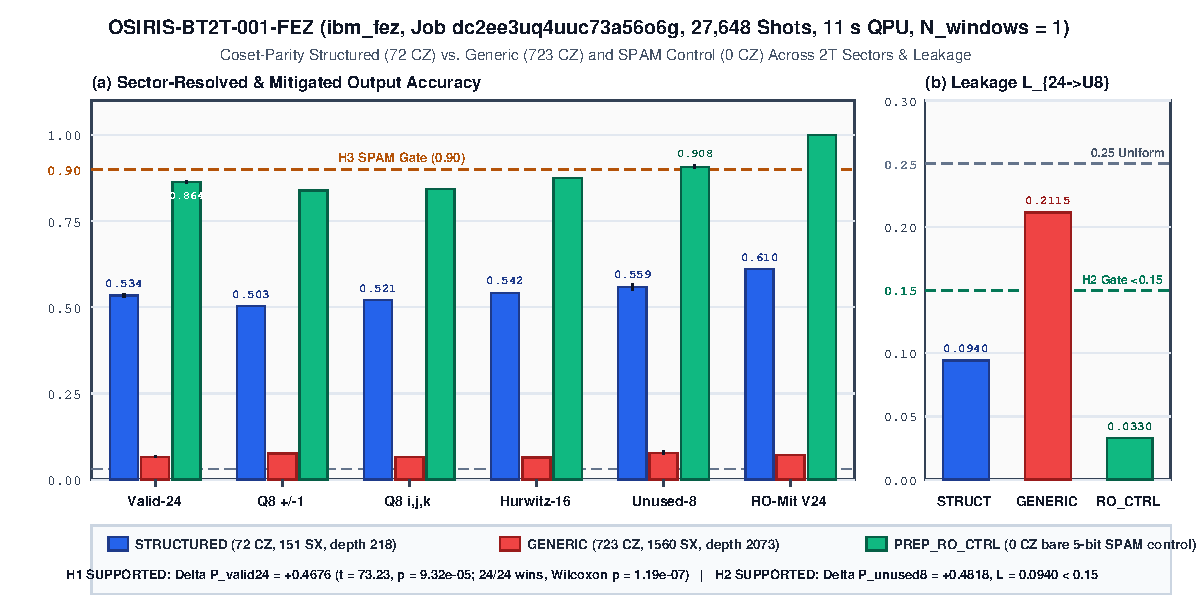
\includegraphics[width=\textwidth]{fig1_bt2t001_fez_synthesis_and_sectors.pdf}
  \caption{Hardware-attested $2T$ inversion benchmark on \btBackend\ (job \btJobId, \btTotalShots\ shots, \btQpuSec\,s QPU, $N_{\mathrm{windows}} = \btCalWindows$). (a)~Comparison of \texttt{STRUCTURED} (\btStructCz\ \texttt{CZ}), \texttt{GENERIC} (\btGenCz\ \texttt{CZ}), and \texttt{PREP\_RO\_CTRL} (\btCtrlCz\ \texttt{CZ}) across uniform valid-$24$, $Q_8$ center $\{\pm\mathbf{1}\}$, $Q_8$ imaginary $\{\pm\mathbf{i},\pm\mathbf{j},\pm\mathbf{k}\}$, Hurwitz-$16$ cosets, unused-$8$ fixed codewords, and $M_{32}$-mitigated valid-$24$ accuracy relative to the $\btHThreeSpamThresh$ \texttt{H3} SPAM gate and $1/32 = \btRandChanceFour$ uniform baseline. (b)~Valid-to-unused subspace leakage $\widehat{L}_{24\to\mathrm{unused}}$ against the $8/32 = \btRandLeakBase$ random baseline and $\btHTwoLeakThresh$ \texttt{H2} confinement threshold.}
  \label{fig:bt2t_sectors}
\end{figure*}

\begin{table*}[t]
\caption{Three-arm hardware results on \btBackend\ T-junction $\btLayoutStr$ (job \btJobId, raw archive SHA-256 prefix \btRawGzSha; $\btShotsPerCell$ equal shots per basis cell across $\btNumBlocks$ blocks; $N_{\mathrm{windows}} = \btCalWindows$). Sampling standard errors reflect within-window binomial uncertainty; inter-block dispersion is reported separately via block values and block SD.}
\label{tab:bt2t_hardware}
\begin{ruledtabular}
\begin{tabular}{lrrrrrrrrr}
Arm (\texttt{CZ} / $\sqrt{X}$ / Depth) & $\widehat{P}_{\mathrm{valid\text{-}24}} \pm \mathrm{SE}$ & Block SD & RO-Mit V24 & $Q_8$ $\{\pm\mathbf{1}\}$ & $Q_8$ $\{\pm\mathbf{i},\mathbf{j},\mathbf{k}\}$ & Hurwitz-16 & $\widehat{P}_{\mathrm{unused\text{-}8}} \pm \mathrm{SE}$ & $\widehat{L}_{24\to\mathrm{unused}}$ & Modal ($32$) \\
\hline
\btTableHardwareSummaryRows
\end{tabular}
\end{ruledtabular}
\end{table*}

Job \btJobId\ executed all $\btTotalPubs$ ISA circuits on \btBackend\ in \btQpuSec\,s of QPU charge time (\btResUnits\ resource units, reducing Open Plan remaining quota from \btQuotaRemBeforeSec\,s to \btQuotaRemAfterSec\,s out of \btQuotaLimitSec\,s). Figure~\ref{fig:bt2t_sectors} and Table~\ref{tab:bt2t_hardware} summarize the three arms across algebraic sectors.

\paragraph{Hypothesis \texttt{H1} (\btHOneVerdict): Structured vs.\ generic valid-$2T$ inversion.}
Compressing the heavy-hex unitary core from \btGenCz\ to \btStructCz\ \texttt{CZ} gates raises raw uniform valid-$24$ inversion probability more than eightfold from $\widehat{P}_{\mathrm{valid\text{-}24}}(\mathrm{GENERIC}) = \btPValidGenRaw \pm \btPValidGenSe$ (blocks $[\btPValidGenBlkZero, \btPValidGenBlkOne, \btPValidGenBlkTwo]$, block SD $\btPValidGenSd$) to $\widehat{P}_{\mathrm{valid\text{-}24}}(\mathrm{STRUCTURED}) = \btPValidStructRaw \pm \btPValidStructSe$ (blocks $[\btPValidStructBlkZero, \btPValidStructBlkOne, \btPValidStructBlkTwo]$, block SD $\btPValidStructSd$). The raw gain $\Delta\widehat{P}_{\mathrm{valid\text{-}24}} = +\btDeltaValidRaw$ exceeds the $\btHOneThresh$ preregistered threshold in every temporal block ($[\btBlkDeltaZero, \btBlkDeltaOne, \btBlkDeltaTwo]$, paired block $t_{\mathrm{df}=2} = \btPairedBlockT$, one-sided $p = \btPairedBlockP$). Across the $\btGroupOrder$ group elements, \texttt{STRUCTURED} strictly outperforms \texttt{GENERIC} on $\btElemWins / \btGroupOrder$ inputs with elementwise gains spanning $+\btElemMinDelta$ to $+\btElemMaxDelta$ (exact two-sided Wilcoxon signed-rank $p = \btWilcoxonP$). Moreover, \texttt{STRUCTURED} maintains uniform fidelity across $Q_8$ center ($\btStructSecCenter$), $Q_8$ imaginary ($\btStructSecImag$), and Hurwitz-$16$ coset ($\btStructSecHurwitz$) sectors, recovers the exact algebraic inverse as the empirical modal bitstring on $\btPValidStructModal / \btGroupOrder$ valid inputs (versus $\btPValidGenModal / \btGroupOrder$ for \texttt{GENERIC}), and rises to $\btPValidStructMit$ under $M_{32}$ readout mitigation (widening the mitigated contrast against \texttt{GENERIC}'s $\btPValidGenMit$ to $+\btDeltaValidMit$).

\paragraph{Hypothesis \texttt{H2} (\btHTwoVerdict): Unused-codeword preservation and subspace confinement.}
On the eight unused codewords $x \in \{24,\dots,31\}$, \texttt{STRUCTURED} achieves $\widehat{P}_{\mathrm{unused\text{-}8}} = \btPUnusedStructRaw \pm \btPUnusedStructSe$ (\btPUnusedStructMit\ readout-mitigated; $\btPUnusedStructModal / \btUnusedCount$ modal matches) versus $\btPUnusedGenRaw \pm \btPUnusedGenSe$ (\btPUnusedGenMit\ mitigated; $\btPUnusedGenModal / \btUnusedCount$ modal matches) for \texttt{GENERIC}, yielding $\Delta\widehat{P}_{\mathrm{unused\text{-}8}} = +\btDeltaUnusedRaw > \btHTwoDeltaThresh$. Valid-to-unused subspace leakage is suppressed to $\widehat{L}_{24\to\mathrm{unused}}(\mathrm{STRUCTURED}) = \btLeakStruct < \btHTwoLeakThresh$, well below both the $8/32 = \btRandLeakBase$ maximally depolarized baseline and \texttt{GENERIC}'s $\btLeakGen$ (while unused-to-valid leakage drops from $\btLeakUnusedToValidGen$ in \texttt{GENERIC} to $\btLeakUnusedToValidStruct$ in \texttt{STRUCTURED}).

\begin{figure*}[t]
  \centering
  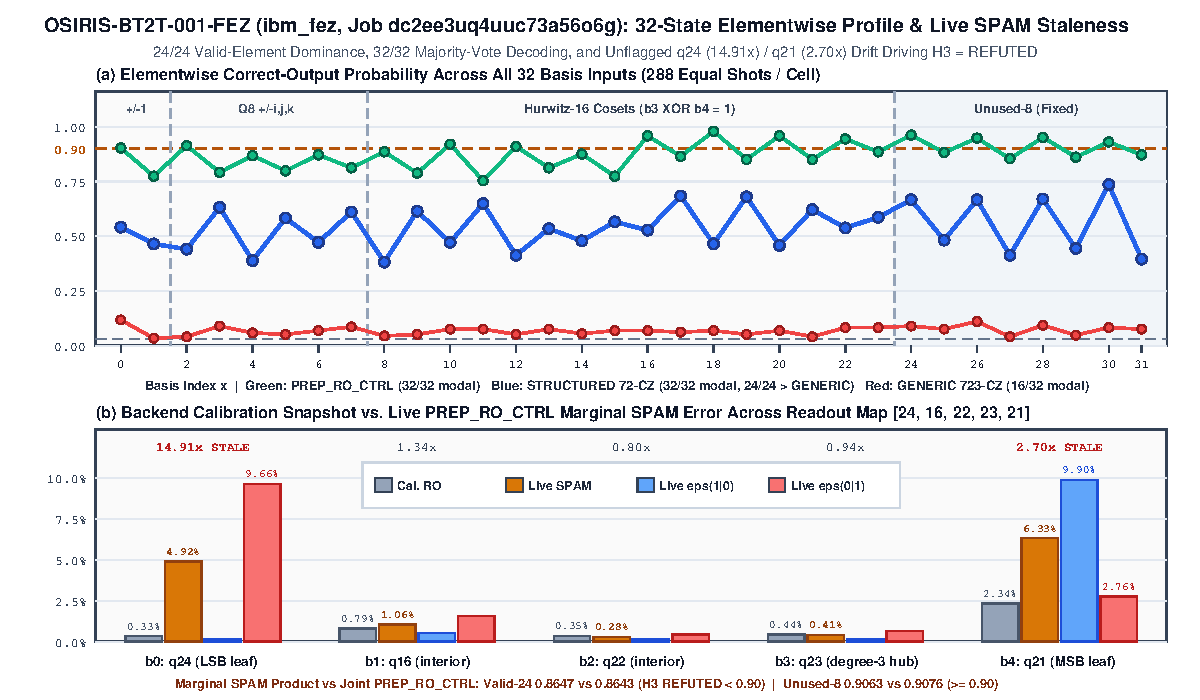
\includegraphics[width=\textwidth]{fig2_bt2t001_fez_elementwise_and_spam_drift.pdf}
  \caption{Elementwise $32$-state inversion profile and live SPAM calibration-staleness attribution on \btBackend\ (job \btJobId). (a)~Raw correct-output probability across all $\btHilbertDim$ basis inputs ($x \in \{0,\dots,23\}$ valid $2T$ elements and $x \in \{24,\dots,31\}$ unused codewords; $\btShotsPerCell$ shots/cell), demonstrating $\btElemWins / \btGroupOrder$ elementwise dominance of \texttt{STRUCTURED} over \texttt{GENERIC}, $\btStructModalAll / \btHilbertDim$ modal majority-vote exact decoding, and systematic odd-$x$ ($b_0=1$ on \texttt{q24}) plus lower-half ($b_4=0$ on \texttt{q21}) sawtooth modulation in \texttt{PREP\_RO\_CTRL}. (b)~Backend-reported readout error versus live \texttt{PREP\_RO\_CTRL} marginal SPAM rates ($\btShotsPerArm$ shots/qubit) across $\btReadoutOrderStr$, isolating the unflagged \btQTwentyFourStaleX\ excursion on \texttt{q24} and \btQTwentyOneStaleX\ excursion on \texttt{q21} that triggered \texttt{H3} = \btHThreeVerdict.}
  \label{fig:bt2t_elementwise_spam}
\end{figure*}

\begin{table}[b]
\caption{Per-transmon backend calibration snapshot versus live \texttt{PREP\_RO\_CTRL} marginal SPAM error rates ($\btShotsPerArm$ shots per qubit across $\btHilbertDim$ basis states) on $\mathrm{T5}$ readout mapping $c[q] \leftarrow \mathrm{T5}[\sigma_{\mathrm{final}}^{\mathrm{struct}}(q)] = \btReadoutOrderStr$.}
\label{tab:bt2t_spam}
\begin{ruledtabular}
\begin{tabular}{llrrrrrr}
Bit & Qubit & $T_1 / T_2$ ($\mu$s) & Cal.\ RO & Live SPAM & $\epsilon(1|0)$ & $\epsilon(0|1)$ & Staleness \\
\hline
\btTablePerQubitSpamRows
\end{tabular}
\end{ruledtabular}
\end{table}

\paragraph{Hypothesis \texttt{H3} (\btHThreeVerdict): Unflagged leaf-qubit SPAM staleness and non-confounding of \texttt{H1}/\texttt{H2}.}
Based on the staging calibration snapshot, independent-qubit readout error predicted a five-bit SPAM baseline of $\prod_{q \in \mathrm{T5}}(1 - \epsilon_{\mathrm{cal}}(q)) = \btCalProdFid$ (\btCalProdFidPct), comfortably above the preregistered $\btHThreeSpamThresh$ \texttt{H3} gate. In live execution, however, \texttt{PREP\_RO\_CTRL} recorded $\widehat{P}_{\mathrm{unused\text{-}8}} = \btPUnusedCtrlRaw \pm \btPUnusedCtrlSe \ge \btHThreeSpamThresh$ but $\widehat{P}_{\mathrm{valid\text{-}24}} = \btPValidCtrlRaw \pm \btPValidCtrlSe < \btHThreeSpamThresh$ (blocks $[\btPValidCtrlBlkZero, \btPValidCtrlBlkOne, \btPValidCtrlBlkTwo]$, block SD $\btPValidCtrlSd$, all-$32$ mean $\btCtrlAllMean$), refuting \texttt{H3}.

Decomposing the $\btShotsPerArm$ \texttt{PREP\_RO\_CTRL} shots into single-qubit bit-flip marginals $\epsilon_q(1|0)$ and $\epsilon_q(0|1)$ (Figure~\ref{fig:bt2t_elementwise_spam}b and Table~\ref{tab:bt2t_spam}) pinpoints the exact physical mechanism. While interior transmons \texttt{q16} (\btQSixteenCalPct\ $\to$ \btQSixteenLivePct, \btQSixteenStaleX), \texttt{q22} (\btQTwentyTwoCalPct\ $\to$ \btQTwentyTwoLivePct, \btQTwentyTwoStaleX), and hub \texttt{q23} (\btQTwentyThreeCalPct\ $\to$ \btQTwentyThreeLivePct, \btQTwentyThreeStaleX) tracked published calibration closely, outer leaf transmon \texttt{q24} (readout bit $b_0$) exhibited an unflagged \btQTwentyFourStaleX\ live SPAM excursion (\btQTwentyFourCalPct\ published versus \btQTwentyFourLivePct\ live, driven by $|1\rangle \to |0\rangle$ relaxation/readout error $\epsilon(0|1) = \btQTwentyFourErrOneZeroPct$ versus $\epsilon(1|0) = \btQTwentyFourErrZeroOnePct$), and outer leaf \texttt{q21} (readout bit $b_4$) exhibited a \btQTwentyOneStaleX\ excursion (\btQTwentyOneCalPct\ published versus \btQTwentyOneLivePct\ live, driven by $|0\rangle \to |1\rangle$ false excitation $\epsilon(1|0) = \btQTwentyOneErrZeroOnePct$ versus $\epsilon(0|1) = \btQTwentyOneErrOneZeroPct$).

This state-asymmetric leaf drift explains both features of Figure~\ref{fig:bt2t_elementwise_spam}a quantitatively. First, the independent single-qubit marginal product
\begin{equation}
  \widehat{P}_{\mathrm{marg}}(x) = \prod_{q=0}^{4} \Bigl(1 - \widehat{\epsilon}_q\bigl(\neg b_q \mid b_q\bigr)\Bigr)
  \label{eq:marginal_product}
\end{equation}
predicts $\btMargPredValid$ on valid-$24$, $\btMargPredUnused$ on unused-$8$, and $\btMargPredAll$ across all $\btHilbertDim$ inputs---matching empirical five-bit joint \texttt{PREP\_RO\_CTRL} accuracies to $|\Delta| = \btMargDiffValid$ on valid-$24$ and $\btMargDiffAll$ across all $\btHilbertDim$ states, ruling out correlated five-qubit readout crosstalk and corroborating our multi-processor Heron~r2 calibration-staleness study (\texttt{RO-06}/\texttt{RO-07})~\cite{DavisRO0607Zenodo2026,DavisTMAP02Zenodo2026}. Second, sixteen of the twenty-four valid $2T$ inputs ($x \in \{0,\dots,15\}$) prepare $b_4 = 0$ on \texttt{q21} (incurring the $\btQTwentyOneErrZeroOnePct$ false-excitation penalty), whereas all eight unused codewords ($x \in \{24,\dots,31\}$) prepare $b_4 = 1$ (incurring only $\btQTwentyOneErrOneZeroPct$), accounting for the gap between $\btPValidCtrlRaw$ and $\btPUnusedCtrlRaw$. Crucially, \texttt{H3} refutation does not confound \texttt{H1} or \texttt{H2}: (i)~all three arms share the identical five physical transmons interleaved inside every temporal block, (ii)~excess SPAM noise strictly attenuates raw \texttt{STRUCTURED} accuracy ($\btPValidStructRaw \to \btPValidStructMit$ after well-conditioned $M_{32}$ inversion, widening the synthesis gap from $+\btDeltaValidRaw$ to $+\btDeltaValidMit$), and (iii)~the tenfold \texttt{CZ} reduction ($\btGenCz \to \btStructCz$) dominates circuit decoherence by nearly an order of magnitude above single-qubit SPAM.

\section{Conclusion}
Aligning finite-group binary encodings with normal-subgroup coset parities transforms exact non-abelian group inversion on $2T \subset SU(2)$ from an impractical $\btGenCz$-\texttt{CZ} truth-table circuit into a compact $\btStructCz$-\texttt{CZ} heavy-hex primitive (\btTkStructZzOpt\ \texttt{ZZPhase} on all-to-all trapped-ion targets) achieving $\btStructModalAll / \btHilbertDim$ exact majority-vote recovery and a $+\btDeltaValidRaw$ raw ($+\btDeltaValidMit$ readout-mitigated) valid-group fidelity gain on \btBackend. At the same time, pairing every algebraic benchmark with an equal-shot interleaved $0$-\texttt{CZ} SPAM control across all $2^n$ basis states proves essential on contemporary superconducting processors: live single-qubit readout excursions up to \btQTwentyFourStaleX\ above static calibration snapshots occur inside normal calibration windows and must be audited transparently via preregistered SPAM gates rather than absorbed into uncalibrated circuit error models.

\begin{acknowledgments}
We acknowledge the use of IBM Quantum services for this work. The views expressed are those of the author and do not reflect the official policy or position of IBM or the IBM Quantum team.
\end{acknowledgments}

\section*{Data and Code Availability}
Write-ahead preregistration (\btPreregSha), independent \texttt{G1} review (\btGoneSha), frozen QPY ISA circuits (\btQpySha), raw $\btTotalPubs$-PUB shot counts (\btRawGzSha), calibration and job receipts (\btJobId), and the RFC~8785 reproducibility capsule (\btCapsuleSha) are archived under \texttt{experiments/bt2t\_inversion/}, \texttt{experiments/bt2t\_fez/}, and \texttt{papers/bt2t001\_binary\_tetrahedral\_fez/}.

\begin{thebibliography}{9}
\bibitem{LammLawrenceYamauchi2019} H. Lamm, S. Lawrence, and Y. Yamauchi (NuQS Collaboration), Phys. Rev. D \textbf{100}, 034518 (2019).
\bibitem{BenderZoharCirac2018} J. Bender, E. Zohar, A. Farace, and J. I. Cirac, New J. Phys. \textbf{20}, 093001 (2018).
\bibitem{MochxonKitaevPreskill2004} C. Mochon, Phys. Rev. A \textbf{69}, 032306 (2004).
\bibitem{Barenco1995} A. Barenco, C. H. Bennett, R. Cleve, D. P. DiVincenzo, N. Margolus, P. Shor, T. Sleator, J. A. Smolin, and H. Weinfurter, Phys. Rev. A \textbf{52}, 3457 (1995).
\bibitem{DavisRO0607Zenodo2026} D. P. Davis, \emph{Transient Readout Staleness and Multiplexed Isolation on 156-Qubit IBM Heron r2 Processors (RO-06/RO-07)}, Zenodo (2026), \texttt{doi:10.5281/zenodo.24420902}.
\bibitem{DavisTMAP02Zenodo2026} D. P. Davis, \emph{Calibration-Ranked Layout Sensitivity and Sign Reversal on Superconducting Heavy-Hex Processors (TMAP-02)}, Zenodo (2026), \texttt{doi:10.5281/zenodo.24406426}.
\end{thebibliography}

\end{document}
